%% ----------------------------------------------------------------
%% Thesis.tex -- MAIN FILE (the one that you compile with LaTeX)
%% ---------------------------------------------------------------- 

% Set up the document
\documentclass[a4paper, 11pt, oneside]{Thesis}  % Use the "Thesis" style, based on the ECS Thesis style by Steve Gunn
\graphicspath{{Figures/}}  % Location of the graphics files (set up for graphics to be in PDF format)

% Include any extra LaTeX packages required
\usepackage[square, numbers, comma, sort&compress]{natbib}  % Use the "Natbib" style for the references in the Bibliography
\usepackage{verbatim}  % Needed for the "comment" environment to make LaTeX comments
\usepackage{vector}  % Allows "\bvec{}" and "\buvec{}" for "blackboard" style bold vectors in maths
\hypersetup{urlcolor=blue, colorlinks=true}  % Colours hyperlinks in blue, but this can be distracting if there are many links.

\newcommand{\E}{\mathbf{E}}
\newcommand{\B}{\mathbf{B}}
\newcommand{\EMH}{\mathbf{H}}
\newcommand{\D}{\mathbf{D}}
\newcommand{\F}{\mathbf{F}}
\newcommand{\weightfunc}{\mathbf{W}}
\newcommand{\R}{\mathbf{R}}
\newcommand{\pder}[2][]{\frac{\partial#1}{\partial#2}}
\newcommand{\pdert}[1]{\frac{\partial#1}{\partial t}}
\newcommand{\figref}[1]{figure \ref{#1}}
\newcommand{\ut}{\frac{\partial \mathbf{U}}{\partial t}}
\newcommand{\fk}{\frac{\partial \mathbf{F_k (\mathbf{U})} }{\partial x_k}}
%% ----------------------------------------------------------------
\begin{document}
\frontmatter	  % Begin Roman style (i, ii, iii, iv...) page numbering

% Set up the Title Page
\title  {Thesis Title}
\authors  {\texorpdfstring
            {\href{your web site or email address}{Author Name}}
            {Author Name}
            }
\addresses  {\groupname\\\deptname\\\univname}  % Do not change this here, instead these must be set in the "Thesis.cls" file, please look through it instead
\date       {\today}
\subject    {}
\keywords   {}

\maketitle
%% ----------------------------------------------------------------

\setstretch{1.3}  % It is better to have smaller font and larger line spacing than the other way round

% Define the page headers using the FancyHdr package and set up for one-sided printing
\fancyhead{}  % Clears all page headers and footers
\rhead{\thepage}  % Sets the right side header to show the page number
\lhead{}  % Clears the left side page header

\pagestyle{fancy}  % Finally, use the "fancy" page style to implement the FancyHdr headers

%% ----------------------------------------------------------------
% Declaration Page required for the Thesis, your institution may give you a different text to place here
\Declaration{

\addtocontents{toc}{\vspace{1em}}  % Add a gap in the Contents, for aesthetics

I, AUTHOR NAME, declare that this thesis titled, `THESIS TITLE' and the work presented in it are my own. I confirm that:

\begin{itemize} 
\item[\tiny{$\blacksquare$}] This work was done wholly or mainly while in candidature for a research degree at this University.
 
\item[\tiny{$\blacksquare$}] Where any part of this thesis has previously been submitted for a degree or any other qualification at this University or any other institution, this has been clearly stated.
 
\item[\tiny{$\blacksquare$}] Where I have consulted the published work of others, this is always clearly attributed.
 
\item[\tiny{$\blacksquare$}] Where I have quoted from the work of others, the source is always given. With the exception of such quotations, this thesis is entirely my own work.
 
\item[\tiny{$\blacksquare$}] I have acknowledged all main sources of help.
 
\item[\tiny{$\blacksquare$}] Where the thesis is based on work done by myself jointly with others, I have made clear exactly what was done by others and what I have contributed myself.
\\
\end{itemize}
 
 
Signed:\\
\rule[1em]{25em}{0.5pt}  % This prints a line for the signature
 
Date:\\
\rule[1em]{25em}{0.5pt}  % This prints a line to write the date
}
\clearpage  % Declaration ended, now start a new page

%% ----------------------------------------------------------------
% The "Funny Quote Page"
\pagestyle{empty}  % No headers or footers for the following pages

\null\vfill
% Now comes the "Funny Quote", written in italics
\textit{``Write a funny quote here.''}

\begin{flushright}
If the quote is taken from someone, their name goes here
\end{flushright}

\vfill\vfill\vfill\vfill\vfill\vfill\null
\clearpage  % Funny Quote page ended, start a new page
%% ----------------------------------------------------------------

% The Abstract Page
\addtotoc{Abstract}  % Add the "Abstract" page entry to the Contents
\abstract{
\addtocontents{toc}{\vspace{1em}}  % Add a gap in the Contents, for aesthetics

The Thesis Abstract is written here (and usually kept to just this page). The page is kept centered vertically so can expand into the blank space above the title too\ldots

}

\clearpage  % Abstract ended, start a new page
%% ----------------------------------------------------------------

\setstretch{1.3}  % Reset the line-spacing to 1.3 for body text (if it has changed)

% The Acknowledgements page, for thanking everyone
\acknowledgements{
\addtocontents{toc}{\vspace{1em}}  % Add a gap in the Contents, for aesthetics

The acknowledgements and the people to thank go here, don't forget to include your project advisor\ldots

}
\clearpage  % End of the Acknowledgements
%% ----------------------------------------------------------------

\pagestyle{fancy}  %The page style headers have been "empty" all this time, now use the "fancy" headers as defined before to bring them back


%% ----------------------------------------------------------------
\lhead{\emph{Contents}}  % Set the left side page header to "Contents"
\tableofcontents  % Write out the Table of Contents

%% ----------------------------------------------------------------
\lhead{\emph{List of Figures}}  % Set the left side page header to "List if Figures"
\listoffigures  % Write out the List of Figures

%% ----------------------------------------------------------------
\lhead{\emph{List of Tables}}  % Set the left side page header to "List of Tables"
\listoftables  % Write out the List of Tables

%% ----------------------------------------------------------------
\setstretch{1.5}  % Set the line spacing to 1.5, this makes the following tables easier to read
\clearpage  % Start a new page
\lhead{\emph{Abbreviations}}  % Set the left side page header to "Abbreviations"
\listofsymbols{ll}  % Include a list of Abbreviations (a table of two columns)
{
% \textbf{Acronym} & \textbf{W}hat (it) \textbf{S}tands \textbf{F}or \\
\textbf{LAH} & \textbf{L}ist \textbf{A}bbreviations \textbf{H}ere \\

}

%% ----------------------------------------------------------------
\clearpage  % Start a new page
\lhead{\emph{Physical Constants}}  % Set the left side page header to "Physical Constants"
\listofconstants{lrcl}  % Include a list of Physical Constants (a four column table)
{
% Constant Name & Symbol & = & Constant Value (with units) \\
Speed of Light & $c$ & $=$ & $2.997\ 924\ 58\times10^{8}\ \mbox{ms}^{-\mbox{s}}$ (exact)\\

}

%% ----------------------------------------------------------------
\clearpage  %Start a new page
\lhead{\emph{Symbols}}  % Set the left side page header to "Symbols"
\listofnomenclature{lll}  % Include a list of Symbols (a three column table)
{
% symbol & name & unit \\
$a$ & distance & m \\
$P$ & power & W (Js$^{-1}$) \\
& & \\ % Gap to separate the Roman symbols from the Greek
$\omega$ & angular frequency & rads$^{-1}$ \\
}
%% ----------------------------------------------------------------
% End of the pre-able, contents and lists of things
% Begin the Dedication page

\setstretch{1.3}  % Return the line spacing back to 1.3

\pagestyle{empty}  % Page style needs to be empty for this page
\dedicatory{For/Dedicated to/To my\ldots}

\addtocontents{toc}{\vspace{2em}}  % Add a gap in the Contents, for aesthetics


%% ----------------------------------------------------------------
\mainmatter	  % Begin normal, numeric (1,2,3...) page numbering
\pagestyle{fancy}  % Return the page headers back to the "fancy" style

% Include the chapters of the thesis, as separate files
% Just uncomment the lines as you write the chapters

% Chapter 1

\chapter{Physical Problem} % Write in your own chapter title
\label{Chapter1}
\lhead{Chapter 1. \emph{Physical Problem}} % Write in your own chapter title to set the page header

\section{Problem Description}

\begin{itemize}
	\item what is the problem? (resonant frequencies in a cavity)
	\item how do lasers work? [Maybe]
	\item what is a cavity? where are they used? why do we care?
	\item what is a spectrum - how does the transformation work? what does it mean?
	\item what is a resonant frequency? why are we interested?
	\item industrial relevance - why is there need for research (nano/smaller)
\end{itemize}
\section{Full Maxwells Equations}
\begin{itemize}
	\item specify equations (as a system of differential, linear conservation eqtns)
	\item what is the problem (resonant frequencies in a cavity)
	\item which equations am I using? and why. Curl/Divergence equations
	\item what is a resonant frequency? why are we interested
	\item Differential vs integral formulation
\end{itemize}
$$ \pdert{E_1} = \pder[H_{3}]{x_2} - \pder[H_{2}]{x_3} $$
$$ \pdert{E_2} = \pder[H_{1}]{x_3} - \pder[H_{3}]{x_1} $$
$$ \pdert{E_3} = \pder[H_{2}]{x_1} - \pder[H_{1}]{x_2} $$
$$ \pdert{H_1} = - \pder[E_{3}]{x_2} + \pder[E_{2}]{x_3} $$
$$ \pdert{H_2} = - \pder[E_{1}]{x_3} + \pder[E_{3}]{x_1} $$
$$ \pdert{H_3} = - \pder[E_{2}]{x_1} + \pder[E_{1}]{x_2} $$

The system of equations can be written in 3D as a linear hyperbolic system of conservation equations:

$$
\pder[\mathbf{U}]{t} + \pder[\mathbf{F}_k(\mathbf{U})]{x_k} = \mathbf{S}(\mathbf{U})
$$

where:

$$
\mathbf{U} = \begin{pmatrix}\epsilon \E \\ \mu \mathbf{H} \end{pmatrix}
\mathbf{F_1} = \begin{pmatrix}0 \\ H_3 \\ - H_2 \\ 0 \\ - E_3 \\ E_2 \end{pmatrix}
\mathbf{F_2} = \begin{pmatrix} -H_3 \\ 0 \\ H_1 \\ E_3 \\ 0 \\ - E_1 \end{pmatrix}
\mathbf{F_3} = \begin{pmatrix} H_3 \\ -H_1 \\ 0 \\ -E_2 \\ E_1 \\ 0 \end{pmatrix}
\mathbf{S} = \mathbf{0}
$$

We can approximate the z-dependence of the system as a sinusoidal wave where each component of the system follows a sinusoidal $x_3$ dependence given by:

$$
\mathbf{U}(x,y,z) = \mathbf{U}(x,y) e^{j(\beta t - \omega t)}
$$

The system of equations can be reduced to 2D by specifying an explicit form for $F_3$. The equation above is therefore modified to have only $F_1$ and $F_2$ with an explicit form for $\pder{F_3}$ introduced as a source term of form.

$$
\mathbf{S} = \begin{pmatrix} \beta sin(\omega t - \beta x_3) \\ \beta sin(\omega t - \beta x_3) \\ 0 \\ \beta sin(\omega t - \beta x_3) \\ \beta sin(\omega t - \beta x_3) \\ 0 \end{pmatrix}
$$

\subsubsection{Loss and Gain}
[Maybe this should go in the Full Maxwells Equations bit?] Somewhere I need to discuss semiconductor lasers, how they work and how I use complex,
\begin{itemize}
	\item significance of parameters, complex material parameters
	\item loss and gain
	\item effective refractive index
	\item propagation loss
	\item quality factors
\end{itemize}
\subsection{Boundary Conditions And Initial Conditions}
\begin{itemize}
	\item Interface Boundary constraints + obtaining from integral form of maxwells equations
	\item Radiation BCs (not really appropriate for me - only used in scattering - don't mention)
	\item initial conditions + effect on solution. e.g. modal initial conditions etc
\end{itemize}

$$
\mathbf{n} \times \mathbf{E^L} = \mathbf{n} \times \mathbf{E^R} 
\mathbf{n} \times \mathbf{H^L} = \mathbf{n} \times \mathbf{H^R} 
$$

$$
\mathbf{n} \dot ( \epsilon^L \mathbf{E^L} ) = - \mathbf{n} \dot ( \epsilon^R \mathbf{E^R} )
$$
$$
\mathbf{n} \dot ( \mu^L \mathbf{H^L} ) = - \mathbf{n} \dot ( mu^R \mathbf{H^R} )
$$

% TODO - note in Rubens thesis the last equation contains \epsilon^R\H^R (which is wrong I think)

\subsection{Validity and Scope}
\begin{itemize}
  \item materials (linear, homogenous, isotropic)
	\item fields (slow varying compared to material response)
	\item how do my problems reflect this
\end{itemize}
\subsection{Other Forms of Maxwells Equations}
\subsubsection{2D compact form}
Mention beta for z-dependence
Obtain formulation from 3D. Mention B=0 -> equations decouple into TE/TM mode
\subsubsection{[Incident Wave Formulation]}
\subsection{Relation to Wave Equation and Helmholtz Equation}
Discuss Freq vs Time domain HERE - conclude why, never touch again.
Derivation
\section{Summary} % Introduction
% Chapter 1

\chapter{Numerical Methods} % Write in your own chapter title
%\label{Chapter2}
%\lhead{Chapter 2. \emph{Numerical Methods}} % Write in your own chapter title to set the page header

\section{Motivation}
\subsection{Available Methods}
\begin{itemize}
	\item Finite Difference
	\item Finite Volume
	\item Finite Element
	\item Other High Order competitors to DG
\end{itemize}

Today there are several poular methods for solving maxwells equations. The one in most widespread use is the Yee Scheme [] proposed in which uses a Finite Difference method. This is popular due to its simplicity and low operation count and has been shown to produce good results [].

However since the method uses structured meshes capturing complicated geometrical boundaries can be an issue and lead to staircasing effects.

In order to resolve these issues several techniques have been proposed. Several techniques incorporate a low finite element or finite volume


The past *** year the Yee scheme of FDTD

\subsection{Unstructured Mesh}
\begin{itemize}
	\item justification of using FEM as opposed to finite difference
	\item unstructured mesh vs structured grid - stair-casing/geometric flexibility, refinement to capture solution
	\item why do we need an unstructured mesg
\end{itemize}
% OPTIONS LEFT: FINITE DIFFERENCE, FINITE VOLUME, FINITE ELEMENT
Finite difference schemes seem very promising and are very popular however in many cases these have many limitations. In FDTD the entire computational domain is discretized using a cartesian structured grid. Complex geometrical boundaries or interfaces become hard to capture with structured grids - and improving the approximation of the boundary requires refiniment of the entire grid. Furthermore capturing solutions which are more complex in certain regions again require refinement over the whole domain. Clearly methods which use an unstructured mesh have a clear advantage since the geometry can be captured accurately with only local refinement of the mesh.

\subsection{High Order}
\begin{itemize}
	\item why high order - capture geometric boundaries + soltn
	\item staircasing + non-physical effects
	\item capture geometry
	\item options for high order (i.e. not finite volume)
\end{itemize}
% OPTIONS LEFT: FINITE VOLUME (or other low order meshes), FINITE ELEMENT
The linear approximation of boundaries in low-order schemes has been shown to cause non-physical issues with the solution as a whole []. These low-order approximations of boundaries can include discontinuities in the boundaries themselves or derivaties of the boundaries (staircasing) which can lead to non-physical effects. High-order schemes allow us to approximate boundaries and interfaces with polynomials.

Also low-order methods suffer from issues with numerical disperion and dissipation which can cause significant errors in wave solutions propagated for long periods of time.

\subsection{Limitations of Methods}
\begin{itemize}
	\item Limitations with high order
	\item sparse, global matrix
	\item approximating curved geometries
\end{itemize}
% OPTIONS LEFT: FINITE ELEMENT (HIGH-ORDER)
High-order FEM scheme have several issues having a sparse global matrix which needs to be inverted. The Discontinuous Galerkin method on the other hand has elemental matricies with elements connected by a numerical flux term. This means there are no large global matricies to invert. Also the approximations in high order are better however geometries are approximated by polynomials. This can still cause issues capturing geometries with a high curvature.

\section{Discontinuous Galerkin}
\subsection{Advantages Of Discontinuous Galerkin}
The Discontinuous Galerkin method was first introduced in 1973 by Reed and Hill [W.H. Reed, T.R. Hill, Triangular mesh methods for the neutron transport equation, Los Alamos Scientific Laboratory, 1973 Tech. Rep. LA-UR-73-479] to solve the neutron transport equation.
\begin{itemize}
	\item discuss advantages for wave-dominated problems
	\item how does DG address the issues with FEM
	\item Capturing wave solutions + numerical dissipation
	\item Influence of choice of numerical flux
\end{itemize}
\subsection{Formulation}
The problems we wish to consider can be written in conservation form as:

$$
\ut + \fk  = \mathbf{S(U)}
$$

This can be written in a weak form as:

$$
\int_{\Omega_e} \mathbf{w} \ut d\Omega_e  - \int_{\Omega_e} \frac{\partial \mathbf{w}}{ \partial x_k} \mathbf{F}(\mathbf{U}) d\Omega + \int_{\partial \Omega_e} \mathbf{w} \mathbf{F_n}(\mathbf{U_e}) d\Gamma = \int_{\Omega_e} \mathbf{w} \mathbf{S}(\mathbf{U_e}) d\Omega
$$

$$
\mathbf{u} = \sum^{N}_{j=1} N_j u_j(t)
$$

$$
\mathbf{w} = N_i
$$

\subsubsection{Local Element Equations}
\begin{itemize}
  \item discretised versions of relevant maxwells equations
	\item local matrix + broken space
	\item Nodal vs Modal representation
\end{itemize}
\subsubsection{Numerical Flux}
\begin{itemize}
	\item role of numerical
  \item specify numerical flux %$A_n^{-}[]$
	\item effect for wave domination problems - flow of information, upwind flux
	\item recover global solution
\end{itemize}
\subsection{Implementing Boundary Conditions}
\begin{itemize}
	\item material interfaces (specifically the PEC) - no need for ABC or PML at the moment (I don't use these)
\end{itemize}
\subsubsection{Spatial Discretisation}
\begin{itemize}
	\item discuss types of element...? Affine.
	\item discuss meshing + NEFEM
	\item condition number of a matrix - moving nodes around (reference work)
Reference other work a lot for this...
\end{itemize}
\subsection{Time Integration}
\begin{itemize}
	\item explicit RK4
	\item explicit vs implicit
	\item other time integration options
	\item does this make a difference?
\end{itemize}
\subsection{[Errors and convergence - put this somewhere else]}
\begin{itemize}
  \item order of errors and expected rates of convergence
\end{itemize}
\section{Signal Analysis}
\begin{itemize}
  \item dependence of resolution/cut-off
	\item window functions and blackman envelope [?]
	\item filter diagonalisation method
	\item Modal Shapes - how to obtain modes from resonant frequencies.
  \item possibly a full comparison of the methods can go here...otherwise present the two options and defer discussions of which is better until 2D Plate section.
\end{itemize}
\section{Method Summary}
\begin{itemize}
  \item Summary of approaches to solving the problem
	\item Summary of complete methods to recover resonant frequencies for a given problem
\end{itemize} % Background Theory
% Chapter 1

\chapter{Analytical Investigations} % Write in your own chapter title
\label{Chapter 4}
\lhead{Chapter 4. \emph{Analytical Investigations}} % Write in your own chapter title to set the page header

\section{Mesh Refinement Study for Analytical Solutions}
A study of FFT and FDM methods using an analytical wave shape were performed to try and determine how the method is affected by signal length and mesh interpolation. The waves studied are of the form:
$$
E(x,t) = \sum_i sin(kx - \omega_i t)
$$
Take two spatial points $x_1$ and $x_2$, which are a distance $\Delta x$ appart. Choose a point $x_0$ which is half way between these two points, and represent the value at that point as a linear interpolation of the values at $x_1$ and $x_2$.
$$
E(x_0,t) = \frac{1}{2} \left[ E(x_1,t) + E(x_2,t) \right]
$$

The studies in this section were performed with a single and multiple frequencies ($\omega_i$) however no major differences were found and the results presented here are for f=100 ($\omega = 2 \pi f$);

The idea is then to cary $\Delta_x$ and investigate the effect of the mesh on the signal achieved. This is illustrated in figure \ref{MonitorPointMeshRefinement_waves_in_space} which shows the spatial, analytical waves in space at time $t=0$ and a line showing the linear approximation being used to find the value at $x_0$ for 9 different values of $\Delta x$. These 9 different values of $\Delta x$ will be used throughout the study. Clearly depending on the size of $\Delta x$ there will be a phase difference in the signals between the sampled points at $x_0$, $x_1$ and $x_2$. A very small $\Delta x$ will give a signal shape very close to signal both at $x_1$ and $x_2$. The larger values of $\Delta x$ however give a linear interpolation with a larger phase difference and the phase difference between the wave at point $x_0$ and $x_1$ in space determines the amplitude. Figure \ref{MonitorPointMeshRefinement_waves_in_time} shows analytical values for signals at $x_0$, $x_1$ and $x_2$ while Figure \ref{MonitorPointMeshRefinement_waves_approx_in_time} shows the analytical values at $x_0$ (the same as those in Figure \ref{MonitorPointMeshRefinement_waves_in_time}) compared to the linear interpolations obtained at $x_0$. Figure \ref{MonitorPointMeshRefinement_waves_approx_in_time} shows that the linear interpolations for the selected $\Delta x$ values vary visibly from the analytical values of the waves sampled at the same point. Values of $\Delta x$ in which the points selected are in phase show an interpolated wave which is in phase. Whilst points out of phase show waves with a very different phase and amplitude.

\begin{figure}
    \subfigure[Waves for t=0 in space showing the linear approximation being used for each $\Delta x$.]{
        \includegraphics[width=0.48\textwidth]{Figures/1D_Analytical_Study/MonitorPointMeshRefinement/waves_in_space.png}
        \label{MonitorPointMeshRefinement_waves_in_space}
    }
    \subfigure[This plot shows the exact (analytical) values of the waves sampled in time at points $x_0$ (green), $x_1$ (blue) and $x_2$ (red).] {
        \label{MonitorPointMeshRefinement_waves_in_time}
        \includegraphics[width=0.48\textwidth]{Figures/1D_Analytical_Study/MonitorPointMeshRefinement/waves_in_time.png}
    }
    
    \subfigure[Values obtained at $x_0$ by linear interpolation (blue) and the corrisponding analytical values at $x_0$ (green) for different $\Delta x$.]{
        \label{MonitorPointMeshRefinement_waves_approx_in_time}
        \includegraphics[width=0.48\textwidth]{Figures/1D_Analytical_Study/MonitorPointMeshRefinement/waves_approx_in_time.png}
    }
    \caption{Analytical and interpolated waves in space and time}
    
    \label{MonitorPointMeshRefinement}
\end{figure}

\begin{figure}
    \subfigure[FFT spectrum from waves sampled for 1000 cycles. Waves with different mesh sizes appear to be have different spectral amplitudes.]{
        \includegraphics[width=0.66\textwidth]{Figures/1D_Analytical_Study/MonitorPointMeshRefinement/waves_in_time_fft.png}
    }
    
    \subfigure[Peak frequency error in the two frequency components from the analytical frequency]{
        \includegraphics[width=0.66\textwidth]{Figures/1D_Analytical_Study/MonitorPointMeshRefinement/PeakFreqError.png}
    }
    \caption{Frequencies Calculated from FFT of signal in time obtained from interpolation at various $\Delta x$s}
    \label{MonitorPointMeshRefinement_FFT}
\end{figure}

\section{Timestep Refinement Study for Analytical Solutions}

A the same analytical wave shapes are used
$$
E(x,t) = \sum_f sin(kx - \omega_f t)
$$
where
$$
\omega_f = [ 100, 120, 1000, 500, 300 ]
$$

\begin{figure}
\includegraphics[width=\textwidth]{Figures/1D_Analytical_Study/MonitorPointDtRefinement/waves_in_time.png}
\caption{Original signal in time with red line showing points selected for approximation}
\end{figure}

\begin{figure}
\includegraphics[width=\textwidth]{Figures/1D_Analytical_Study/MonitorPointDtRefinement/waves_in_time_fft.png}
\caption{Spectrum FFT - cut off point visible}
\end{figure}

\begin{figure}
\includegraphics[width=\textwidth]{Figures/1D_Analytical_Study/MonitorPointDtRefinement/PeakFreqError.png}
\caption{Frequencies plotted up to cutoff point}
\end{figure}

\begin{figure}
\includegraphics[width=\textwidth]{Figures/1D_Analytical_Study/MonitorPointDtRefinement_byDoubling/PeakFreqError.png}
\caption{Frequencies plotted against cutoff (more points)}
\end{figure} % Experiment 1
% Chapter 1

\chapter{Numerical FDTD 1D Simulations} % Write in your own chapter title
\label{Chapter5}
\lhead{Chapter 5. \emph{Numerical FDTD 1D Simulations}} % Write in your own chapter title to set the page header

Numerical simulations were performed using a simple finite difference 1D time domain solver by propagating a wave of the form:

$$
sin(2 \pi f (t - x))
$$

The code used was a simple FDTD 1D implementation written in matlab.

The domain used for all simulations was [0,20] and the waves obtained were compared to the analytical solutions to produce an L2 norm of the resulting wave. The initial conditions used were zero in the whole domain and dirichlet boundary conditions were introduced on the left boundary - however as can be noted from the analytical form of the wave this does not introduce a discontinuity in the solution (at least not to first order). No boundary condition is set on the right hand side of the domain - but the simulation was stopped before the wave reached the far side.
All analysis was done on the 3rd component of the TE mode (E3) which is continuous.
%TODO - verify this...!
Unless otherwise specified the frequency used was f=2, the domain used is of length L=100 with final time at 0.9L with the signal captured at x=20.
% TODO - verify this...!

\begin{figure}
\includegraphics[width=\textwidth]{Figures/1D_FD_propagation/L2_norm_only_dt_refinement/aggregate.png}
\caption{Various mesh size were selected and kept constant while dt was refined. The lower bound on dt is set purely by computational time with no stability constraints. The L2 norm error both in the wave shape over the domain at the final time and in a signal sampled at a selected point at intervals of dt is shown.}
\label{dt_refinement}
\end{figure}

\begin{figure}
\includegraphics[width=\textwidth]{Figures/1D_FD_propagation/L2_norm_only_dx_refinement/aggregate_2.png}
\caption{A similar analysis to figure \ref{dt_refinement} shows dx refinement for fixed dt values. In this case the stability condition and the choice of dt sets a lower bound of dt (dt=dx).}
\end{figure}

% \begin{figure}
% \includegraphics[width=\textwidth]{Figures/1D_FD_propagation/L2_norm_only_dx_refinement/aggregate_10.png}
% \caption{dx refinement for various fixed dt values for frequency f=10. Note there is a lower bound of dt=dx in this case for stability.}
% \end{figure}
% 
% \begin{figure}
% \includegraphics[width=\textwidth]{Figures/1D_FD_propagation/L2_norm_only_dx_refinement/aggregate_20.png}
% \caption{dx refinement for various fixed dt values for frequency f=20. Note there is a lower bound of dt=dx in this case for stability.}
% \end{figure}

\begin{figure}
\includegraphics[width=\textwidth]{Figures/1D_FD_propagation/L2_norm_vs_dx_C_0_8/aggregate_2.png}
\caption{The L2 norm error in the wave and signal shapes with uniform dx and dt (by a factor of 2) refinement using a consisten value of C=0.8. The plots are shown against dx however there is also an implied refinement of dt.}
\end{figure}

\begin{figure}
    \begin{center}
        \subfigure[FFT calculations]{
            \label{FTTC}
            \includegraphics[width=0.6\textwidth]{Figures/1D_FD_propagation/Convergence_plots_with_C/error_from_spectrum_vs_c.png}
        }
        
        \subfigure[FDM calculations]{
            \includegraphics[width=0.6\textwidth]{Figures/1D_FD_propagation/Convergence_plots_with_C/error_from_fdm_vs_c.png}
            \label{FDMC}
        }
        \caption{Error in frequency calculation for different values of C. In this case the refinement was performed by setting dx=0.1 and choosing a dt for the selected C. Then allowing uniform refinement of dx and dt simultaneously by a factor of 2 to preserve C.}
    \end{center}
    
\end{figure}


\begin{figure}
\includegraphics[width=\textwidth]{Figures/1D_FD_propagation/Convergence_plots_with_dx/aggregate_2.png}
\caption{This plots show the relative error in frequency converging with dx for selected constant values of dt for a frequency f=2}
\end{figure}

\begin{figure}
\includegraphics[width=\textwidth]{Figures/1D_FD_propagation/Convergence_plots_with_dx/aggregate_20.png}
\caption{This plots show the relative error in frequency converging with dx for selected constant values of dt for a frequency f=20}
\end{figure}

\begin{figure}
\includegraphics[width=\textwidth]{Figures/1D_FD_propagation/Convergence_plots_with_dx/aggregate_10.png}
\caption{This plots show the relative error in frequency converging with dx for selected constant values of dt for a frequency f=10}
\end{figure}

\begin{figure}
\includegraphics[width=\textwidth]{Figures/1D_FD_propagation/PeriodStudy_long_run/FDM_and_FFT_errors.png}
\caption{A brief period study to select the time required for sufficient accuracy of FDM and FFT methods}
\end{figure}
 % Experiment 1
% Chapter 1

\chapter{Numerical DGTD 2D Simulations} % Write in your own chapter title
\label{Chapter6}
\lhead{Chapter 6. \emph{Numerical DGTD 2D Simulations}} % Write in your own chapter title to set the page header

A simple 2D plane wave was propagated in a rectangular free-space 2D waveguide of width 0.5 and length L. All simulations are performed with p=1.
The same timestep was used for all simulations of 0.5E-3 (this is consistent with timectt=0.2 for the smallest element size used) and length of a cycle = 1.

\begin{figure}
\includegraphics[width=\textwidth]{Figures/2D_DGTD_RectWaveGuide/timestepTooLarge/1E-3/storeFrames/pml0.5/L2ConvPlot_pmls_xmax_half_iframe_30.png}
\caption{Domain of size 0.5x0.5 with a PML of length shown in legend after 3 cycles [run too short]}
\end{figure}

\begin{figure}
\includegraphics[width=\textwidth]{Figures/2D_DGTD_RectWaveGuide/timestepTooLarge/1E-3/storeFrames/pml1.5/L2ConvPlot_pml1_point_5_xmax1_iframe100.png}
\caption{Domain of size 0.5x1.5 with a PML of length shown in legend after 10 cycles}
\end{figure}

\begin{figure}
\includegraphics[width=\textwidth]{Figures/2D_DGTD_RectWaveGuide/timestepTooLarge/1E-3/storeFrames/pml1.5/L2ConvPlot_pml1_point_5_xmax0_point_5_iframe100.png}
\caption{L2 norm for domain of size 0.5x1.5 with a PML of length shown in legend with error measured only on interval [0,0.5] again over 10 cycles}
\end{figure}

\begin{figure}
\includegraphics[width=\textwidth]{Figures/2D_DGTD_RectWaveGuide/timestepTooLarge/1E-3/storeFrames/pml1.5/L2ConvPlot_pml1_point_5_xmax1_iframe100.png}
\caption{L2 norm for domain of size 0.5x1.5 with a PML of length shown in legend with error measured only on interval [0,1] again over 10 cycles}
\end{figure}

\begin{figure}
\includegraphics[width=\textwidth]{Figures/2D_DGTD_RectWaveGuide/timestepTooLarge/0.5E-3/p1/0.5x1/L2Conv.png}
\caption{L2 Convergence with time for L=1 with various element refinements. The number of elements is shown in the figure}
\end{figure}

\begin{figure}
\includegraphics[width=\textwidth]{Figures/2D_DGTD_RectWaveGuide/timestepTooLarge/0.5E-3/p1/0.5x1/L2ConvPlot.png}
\caption{Convergence plot with time obtained from the final timestep (T=10) for L=1}
\end{figure}

\begin{figure}
\includegraphics[width=\textwidth]{Figures/2D_DGTD_RectWaveGuide/timestepTooLarge/0.5E-3/p1/0.5x1.5/L2Conv.png}
\caption{L2 Convergence with time for L=1.5 with various element refinements. The number of elements is shown in the figure}
\end{figure}

\begin{figure}
\includegraphics[width=\textwidth]{Figures/2D_DGTD_RectWaveGuide/timestepTooLarge/0.5E-3/p1/0.5x1.5/L2ConvPlot.png}
\caption{Convergence plot with time obtained from the final timestep (T=10) for L=1.5}
\end{figure}

\begin{figure}
\includegraphics[width=\textwidth]{Figures/2D_DGTD_RectWaveGuide/timestepTooLarge/0.5E-3/p1/0.5x1.5_pml/FinalRun_16x48.png}
\caption{Wave shapes and errors for L=1.5 with attempt to introduce PML with 15x48 elements, p=1}
\end{figure}

\begin{figure}
\includegraphics[width=\textwidth]{Figures/2D_DGTD_RectWaveGuide/timestepTooLarge/0.5E-3/p1/0.5x5/L2ConvWithTime.png}
\caption{L2 norm convergence for different number of element with time for L=5. This shows less error due to reflection.}
\end{figure}

\begin{figure}
\includegraphics[width=\textwidth]{Figures/2D_DGTD_RectWaveGuide/timestepTooLarge/0.5E-3/p1/0.5x5/L2ConvWithH.png}
\caption{Convergence of L2 norm for the wave at the final time T=10 with element size h with L=5}
\end{figure}

\begin{figure}
\includegraphics[width=\textwidth]{Figures/2D_DGTD_RectWaveGuide/timestepTooLarge/0.5E-3/p1/0.5x5/FinalRun_16x160.png}
\caption{Numerical solution, Analytical solution and absolute error at every point int he domain for 16x160 elements with L=5}
\end{figure}

\begin{figure}
\includegraphics[width=\textwidth]{Figures/2D_DGTD_RectWaveGuide/timestepTooLarge/0.5E-3/p1/0.5x5/FinalRun_8x80.png}
\caption{Numerical solution, Analytical solution and absolute error at every point int he domain for 8x80 elements with L=5}
\end{figure}

 % Experiment 2
% Chapter 1

\chapter{2D Plate} % Write in your own chapter title
%\label{Chapter3}
\lhead{Chapter 3. \emph{Results}} % Write in your own chapter title to set the page header

\section{Wave behaviour}
% \begin{itemize}
% \item how do I quantify a good wave - is there a correspondence between this convergence and wave shape convergence? So does this mean I can do convergence in terms of wave shapes maybe? EEEEK.
% \item do a LOT of high-p short runs to try and identify a convergence between multiple waves.
% \end{itemize}

% TODO = SAY HOW MANY TIMESTEPS NOT HOW MANY SECONDS....!
All results presented here are generated with compact 2D formulation with an explicit z-dependence. Results for spectrum are generated with propagation constant equal to zero which will match analytical solution for a 2D plate.

Wave shapes obtained as a solution to maxwells equations should converge as a power $p+1$ where p is the order of shape functions used. Figure \figref{WaveConv2} shows the convergence of the wave shape with element size starting from three different initial conditions compared to a reference solution. For a delta initial condition a convergence of 1.9 is obtained after 500 and 1000 seconds. However for the gaussian initial condition the convergence for a narrow gaussian was significantly different with the convergence for a wider gaussian being close to that expected $~ 1.4$.

\begin{figure}
\includegraphics[width=\textwidth]{Figures/matlab/convergence_of_wave_shapes_with_h_100_frames.png}
\caption{L2 norm of wave shape with element size compared to a reference wave. L2 norm is relative to a reference wave with h=0.025}
\label{WaveConv2}
\end{figure}
%TODO - do the plot again with a lower value of h...if possible (only do 50 'frames')

We expect that this is due to the number of points required to accurately capture a gaussian initial condition. In \figref{WaveConv7} and \figref{WaveConv8} we can see wave shapes after 100s for both delta and gaussian initial conditions respectively. We can see visually that at finer mesh refinements the gaussian wave shapes appear to contain higher harmonics. The wave produced from a delta function however does not. Capturing more frequencies will be desirable for capturing a better spectrum and we expect that at further mesh refinement the both wave shapes will converge.

\begin{figure}
\includegraphics[width=\textwidth]{Figures/matlab/WaveShapes/PlotDeltaWaveShapes.png}
\caption{H 3 components obtained after 100s for delta function initial condition for various mesh refinements}
\label{WaveConv7}
\end{figure}

\begin{figure}
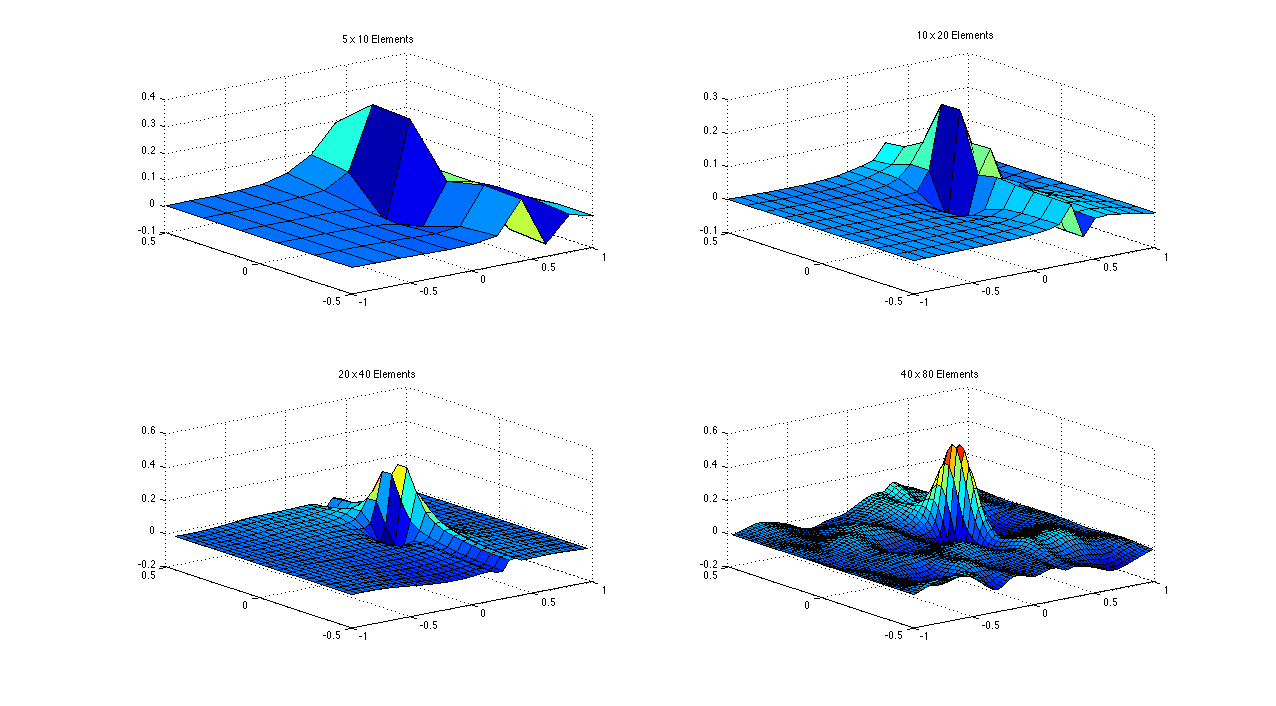
\includegraphics[width=\textwidth]{Figures/waves_in_cavity/waves_in_cavity.png}
\caption{H 3 components obtained after 100 seconds for gaussian function initial condition for various mesh refinements}
\label{WaveConv8}
\end{figure}

\begin{figure}
\includegraphics[width=\textwidth]{Figures/waves_in_cavity/waves_in_cavity_section_delta.png}
\label{WaveConv9}
\end{figure}

\begin{figure}
\includegraphics[width=\textwidth]{Figures/waves_in_cavity/waves_in_cavity_section_gauss.png}
\label{WaveConv10}
\end{figure}


% TODO - non-zero beta values

% TODO - CHECH THAT THIS IS ACTUALLY TRUE

% TODO - 

% TODO - why is this? Are gaussian initial conditions actually better in the long run??

%ConvergeOfWaveShapeWithH:
%-> this was measured after 10 cycles (is that enough for convergence? Who knows?)
%-> NOTE: I NEED TO RUN THIS WITH A HIGHER P AND A BETTER INITIAL CONDITION METHINKS....!! WAAAA!!!

% TODO - EVENTUALLY...! Convergence with P
% \begin{figure}
% \includegraphics[width=\textwidth]{Figures/2DPlate/WaveShapes/ConvergeOfWaveShapeWithP.png}
% \caption{Converge of wave shape with shape function order}
% \label{WaveConv3}
% \end{figure}

% \begin{figure}
% \includegraphics[width=\textwidth]{Figures/matlab/emptyplot.png}
% \caption{Convergence of wave shape measured at a point in space}
% \label{WaveConv4}
% \end{figure}

% \begin{figure}
% \includegraphics[width=\textwidth]{Figures/matlab/emptyplot.png}
% \caption{Error at same point in space as a function of time for various values of p (end every cycle)}
% \label{WaveConv5}
% \end{figure}

% \begin{figure}
% \includegraphics[width=\textwidth]{Figures/matlab/emptyplot.png}
% \caption{Error at same point in space as a function of time for various values of h (end every cycle)}
% \label{WaveConv6}
% \end{figure}

% \subsection{Propagation Constant}
% $\beta$ non-zero runs
% TODO: Change beta and show that the waves change as expected. Try to explain this in terms of the significance of Beta??
% \subsection{conclusion}

\section{FFT Spectrums}

Determination of frequency components of a time domain solution to maxwells equations is commonly done by a fourier transform to frequency space. The following spectrum was obtained by a Discrete Fourier Transform of a signal obtained from a finite element simulation. Peaks corrispond to resonant frequencies - known analytical values for resonant frequency are plotted for comparison.

\begin{figure}
\includegraphics[width=\textwidth]{Figures/matlab/Spectrums/GoodSpectrum.png}
\caption{Spectrum obtained by FFT from a timestep of 0.13E-03, 3,286,002 timesteps and 3200 elements. First order shape functions were used. A blackman window was used to reduce noise.}
\label{Spectrum1}
\end{figure}

% TODO - MAYBE DO WITHOUT A BLACKMAN WINDOW AND WITH A DELTA-FUNCTION INIT COND
% 
% \subsection{Window Functions}
% 
% \begin{figure}
% \includegraphics[width=\textwidth]{Figures/matlab/emptyplot.png}
% \caption{Spectrums with and without a window function}
% \label{WindowFFT1}
% \end{figure}
% 
% Quantify the noise (lowest possible cutoff frequency maybe, or cutoff freq difference)

\subsection{Peak Detection}

\subsubsection{Timestep And Cut-Off Frequencies}

% TODO - higher than Nyquist frequency??

% I need to determine a cut-off frequency?? What strategies do I have?
% 
% plot histogram for various differnt types of spectrum to show differences...! A BAD spectrum should have a BAD histogram
% Plot histogram to a number of ANALYTICAL frequencies with different samplings and spectrum richness (maybe) ??

The highest frequency component which can be indentified from a time-domain signal sampled at frequency $f_{s} = \frac{1}{T}$ where $T$ is the sampling time interval is given by:

$$f_{max} = \frac{f_s}{2} = \frac{1}{2T} $$

This introduces a theoretical upper bound on the spectrum obtained based on sampling frequency. In practice since the sampling interval used is the simulation time step then an upper limit will also be imposed by the stability criterion:

% TODO: STABILITY CRITERION

In practice upper limit for a wave domainated simulation will be the same as the time integration timestep of the simulation which is governed by stability conditions.

However as can be seen in \figref{Timestep1} a finite time-domain signal a sufficiently high sampling frequency will also introduces signal noise below this limit. Here the theoretical highest frequency is shown for each plot however we see degredation in the quality of the spectrum below this cut-off frequency. A sufficiently small timestep should be selected to allow the peaks to be clearly distingushed from spectrum noise. A practical measure of this degredation could be ratio of maximum height of spectral noise to minimum height of signal as shown in \figref{Timestep01}. 

%TODO - show this stuff for HARMINV too (to demonstrate that its relevant).

%TODO:CHECK THIS statement
In practice for these simple examples the time step required for solution stability was sufficient to identify the fundamental frequency of interest. However this could be a consideration if frequencies of interest were higher. %TODO - quantify this...! How much higher before it becomes comparible to stability

%TODO: QUANTIFY how much the timestep effects the ACTUAL frequencies (i.e. by finding the CLOSEST PEAK) - because the input signal is the same every time this probably won't be affected too much by frequency %(dt) for a long run. The real difficulty is in identifying the real and fictitious peaks which arise in the frequency determination. 

\begin{figure}
\includegraphics[width=\textwidth]{Figures/matlab/TimestepConvergence/Spectrums4up.png}
\caption{Spectrum obtained from the same signal using different sampling rates. Signal was generated with a 3200 element mesh and p-2 shape functions and a final time of 500s. The lowest sampling frequency corrisponds to the simulation timestep}
%TODO - how many elements.
%TODO - graph titles
\label{Timestep1}
\end{figure}

%TODO: Talk about cutoff frequencies and identifying resonant frequencies. Noise appears. How does this change with time. If I take a longer time for a noisy signal will this get better?

\begin{figure}
\includegraphics[width=\textwidth]{Figures/matlab/TimeStepConvergence/TimeStepConv.png}
\caption{Error in resonant frequency maximum against sampling period. Same signal used as in \figref{Timestep1}.}
%TODO - how many elements.
%TODO - graph titles
\label{Timestep01}
\end{figure}

%TODO - do this...!
%\begin{figure}
%\includegraphics[width=\textwidth]{Figures/matlab/emptyplot.png}
%\caption{Ratio of minimum resonant frequency component to maximum noise for the first 3 frequencies vs sampling frequency. Same signal used as in \figref{Timestep1}.}
% [or some other measure of how easy it is to extract frequencies - maybe based on histograms?? ]
%\label{Timestep0}
%\end{figure}

% \begin{figure}
% \includegraphics[width=\textwidth]{Figures/matlab/emptyplot.png}
% \caption{Frequencies obtained by sampling a analytical generated spectrum}
% \label{Timestep3}
% \end{figure}

\subsubsection{Peak Resolution}
Signals of finite length undergo a spectral leakage under fourier transform. As a result a shorter sample length results in noise appearing in the a spectrum with wider, badly-resolved peaks as shown in \figref{Period1}. A signal of length $5 \times 10^4$ is sufficient to capture the resonant frequencies with an error of $3 \times 10^6$.

%What is the minimum time I need to accurately capture ths signal at the accuracy required?
% note: more accuracy MEANS that we need much longer runs. No good having a more accurate wave...we also need a more accurate FFT...! So to capture a p3 accuracy with the same level of accuracy we need to run for how many time longer?? :)

% TODO Whats the minimum time (in general) that I need to remove the FFT transform error completely? :)

% TODO: Expression of dependence between timestep and resolution

\begin{figure}
\includegraphics[width=\textwidth]{Figures/matlab/PeriodConvergence/Spectrums4up.png}
\caption{Spectrum obtained from signal using different signal periods. Signal were generated with a timestep of 0.95E-02 using a mesh of 200 elements and p-1 shape functions}
\label{Period1}
\end{figure}

\begin{figure}
\includegraphics[width=\textwidth]{Figures/matlab/PeriodConvergence/PeriodConvergenceManual.png}
\caption{Error in calulations of resonant frequencies obtained against signal length}
\label{Period2}
\end{figure}

%TODO - same for analytical signals made of 1,3,10 \& 100 frequency components
%Use an analytical soltuion to identify (depending on richness of spectrum) the kind of accuracy I can expect to obtain after a FFT.

\subsubsection{Lorentzian Fitting}

In \figref{LorentzFit1} we see a number of resonant peaks fitted with a Lorentzian curve given by:

$$
L(x)=\frac{1}{\pi} \frac{\frac{1}{2}\Gamma}{ (x-x_0)^2 + (\frac{1}{2}\Gamma)^2}
$$

where $x_0$ is the center and $\Gamma$ is a width parameter. The Lorentzian function is commonly used to overcome the peak broadening associated with spectral leakage. In practice however fitting a lorentz curve reliably for narrow peak widths using a least squares method was complicated. However for peaks with less a bad resolution an improvement in the resolution was observed as shown in \figref{LorentzFit2}. This difficulty with fitting is one of the motivations for using the Filter Diagonalisation Method presented later.

\begin{figure}
\includegraphics[width=\textwidth]{Figures/matlab/Lorentz/LorentzFitManual.png}
\caption{Resonant peaks fitted with Lorentz curve at various periods showing the lorentz curve fits as spectrum resolution increases}
\label{LorentzFit1}
\end{figure}

\begin{figure}
\includegraphics[width=\textwidth]{Figures/matlab/Lorentz/LorentzFitPeriodConv.png}
\caption{Results showing the difference obtained by using a Lorentz fit at low periods. Resonably results can be obtained from very short runs in this way. However for longer runs the lorentz fit implementation was less reliable.}
\label{LorentzFit2}
\end{figure}

%\subsection{Spectral Richness}
%Dependece of spectral richness on initial conditions. Dependence of peak height and sharpness on intial conditions too [ maybe this should go somewhere else]

\begin{figure}
\includegraphics[width=\textwidth]{Figures/matlab/harminvr/InitCondHarminv.png}
\caption{Error vs Time for different types of initial conditions produced with FDM method}
\label{InitCond1}
\end{figure}
%delta/gaussian/multiple gaussians(10)/narrow gaussians

%Initial Condition Optimisation:
%\begin{figure}
%\includegraphics[width=\textwidth]{Figures/matlab/emptyplot.png}
%\caption{L2 norm error in the wave shapes against time for different types of initial conditions}
%\label{InitCond2}
%\end{figure}

% \subsubsection{Symmetry}
% \begin{figure}
% \includegraphics[width=\textwidth]{Figures/matlab/emptyplot.png}
% \caption{Spectrum from point with low symmetry and spectrum obtained from same simulation at a point with a high symmetry}
% \label{SymmDep1}
% \end{figure}

% Mesh dependence of initial condition:
% \begin{figure}
% \includegraphics[width=\textwidth]{Figures/matlab/emptyplot.png}
% \caption{Wave vs time for the same gaussian with different mesh sizes}
% \label{SymmDep2}
% \end{figure}

% TODO: Discussion on how finer meshes can capture a better spectrum due to initial condition containing a richer spectrum.

%\subsubsection{Components}
%
%\begin{figure}
%\includegraphics[width=\textwidth]{Figures/matlab/emptyplot.png}
%\caption{Spectrums obtained after 15 cycles}
%\label{CompDep2}
%\end{figure}

% TODO: Different components dominate in different cycles. Can I change the initial conditions to affect this?
%TODO - try to show that spectrums are richer for narrower gaussians??
%TODO(maybe): excite a single component... (?)

%\subsection{Obtaining Data}
%Quality factor...? Should I even mention this?

%\subsection{Conclusion}
%Limitations of FFT. Advantages of FFT (can see the spectrum)

\section{Filter Diagonalization Method}

% V. A. Mandelshtam and H. S. Taylor, "Harmonic inversion of time signals," J. Chem. Phys. 107 (17), 6756-6769 (1997). Erratum, ibid. 109 (10), 4128 (1998).
Limitations with FFT include the number of cycles required for optimal accuracy and the difficulty of lorentz fitting as the peak width gets narrower. The Filter Diagonalization is a popular method that addresses these issues and produces good results in much shorter times. The following are a list of results obtained using the Filter Diagonalization Method. However it is sometimes desirable to also use FFT in order to have a visible spectrum and a more complete picture of spectral content.

Signals were found to sometimes contain additional frequencies or to miss frequencies - but this could be corrected by using a higher number of basis functions.

%when signal consists of arbitrary number...
%TODO - getting rid of additional modes. When do these addtional modes appear? What happens if a run is too long? What happens if its too short.
%--> We get the Q for free (HOOOOW???)

% \begin{figure}
% \includegraphics[width=\textwidth]{Figures/matlab/emptyplot.png}
% \caption{Good spectrum and results obtained from FDM}
% \label{HarmivSpectrum1}
% \end{figure}
% 
% \begin{figure}
% \includegraphics[width=\textwidth]{Figures/matlab/emptyplot.png}
% \caption{Bad spectrum and results obtained from FDM method}
% \label{HarmivSpectrum2}
% \end{figure}
% TODO  FDM and how to optimise. Discuss crap spectrums producing usable results. Discuss fictitious/additional modes and how to get rid of them.......!!

\begin{figure}
\includegraphics[width=\textwidth]{Figures/matlab/harminvr/ConvergenceForDifferentDtHarminv.png}
\caption{Convergence of FDM results for various signal lengths for two different sampling intervals. Note that these sampling intervals also corrispond to time integration timestep. Results are compared with convergence results obtained from the same data for FFT.}
\label{HarmivSpectrum3}
\end{figure}

\begin{figure}
\includegraphics[width=\textwidth]{Figures/matlab/harminvr/HarminvConvergencePlots.png}
\caption{Error in FDM calculations obtained by mesh refinement using 50, 200 and 800 elements for p1 calculations}
\label{HarmivSpectrum4}
\end{figure}

%TODO - Harminv is x times better. Compare them...! Identifying fictitious modes

%\subsection{Initial Condition Dependence}
%show different initial conditions (gaussian, delta, sigma, number of gaussians) - same plot as before with Harminv. Demonstrate difference in initial conditions.

%TODO: is FDM more or less sensitive to initial condition time steps?

%\subsection{Window Functions}

% \begin{figure}
% \includegraphics[width=\textwidth]{Figures/matlab/emptyplot.png}
% \caption{Convergence with window length}
% \label{HarmivWindow1}
% \end{figure}

% \begin{figure}
% \includegraphics[width=\textwidth]{Figures/matlab/emptyplot.png}
% \caption{Convergence with window start time for different p/h}
% \label{HarmivWindow2}
% \end{figure}
 % Experimental Setup
% Chapter 1

\chapter{Dispersive Materials} % Write in your own chapter title
\label{Chapter4}
\lhead{Chapter 3. \emph{Dispersive Materials}} % Write in your own chapter title to set the page header

In general light travels as a polychromatic waves - containing several different frequencies. In general each frequency travels at a different speed in a medium. The material parameters depend on the frequency of the radiation.

\section{The Drude Model}

The drude model was initially proposed in *** based on the kinetic theory of gases [citation]. In the drude model a metal is modelled as a fixed lattice of positively charged ions in a sea of negatively charged valance or conduction (in a metal) electrons which are free to move.

%TODO  - direct quote - IntriaPaper DGTD dispersive
Assumptions:
• The electrons description is non-relativistic;
• The only considered interactions are the electron/wave and the electron/ion ones;
• The electron/ion collisions are instantaneous and random events, and their probability of happening during a dt amount of time is equal to dt 1;
τf
• After an electron/ion collision, the new velocity and direction of the electron are inde-
pendant of those before the collision.


Under these hypotheses, the frequency dependence of the medium permittivity can be de- duced from the equations of motion.
%TODO - end direct quote

When subjected to a constant external electric field $\mathbf{E}$ the displacement of the heavy valence ions from their equilibtrium position is assume to be negligable whilst the electrons move significantly from their equilibrium position in response to an externally applied field. This results in an additional electric field $\mathbf{P}$ due to material response to the applied field $\mathbf{E}$ orientated in the opposite direction resulting in a total field given by the electric displacement field $\mathbf{D}$ where:

$$
\mathbf{D} = \epsilon_0 \mathbf{E} + \mathbf{P}
$$

Note that usually the signs of $\mathbf{P}$ and $\mathbf{E}$ will be opposite - resulting in an induced field that opposes the applied field and consequentially a reduced field in the medium.

% TODO: Is it accurate to describe the displacement electric field as the total electric field....?

For a constant or slow-varying field with respect to the material response time $\tau$ the polarisation of the material $\mathbf{P}$ will be proportional to the applied electric field and can be described as a constant of proportionality $\chi$, known as the electric susceptibility which describes how susceptible the material is to polarisation. $\mathbf{P}$ can be written as:

$$
\mathbf{P} = \chi \mathbf{E}
$$

$\chi$ is not always constant - and in general is a tensor.

Furthermore the movement of electrons from their zero-field equlibrium positions to the equilibrium positions under the applied field $\mathbf{E}$ could take some finite time $\tau$ (characteristic time). For an applied electric field $\mathbf{E}$ which is changing sufficiently quickly this time needs to be accounted for and $\chi$ may not be described as simply by a constant since it clearly depends on the history of the mediums polarisation.

TODO - derivation from equations of motion to conservation form....find a nice way of doing this....

\section{Beyond the Drude Model}
- what about the Lorentz model
- Drude/Lorentz model
- Debye model
- Generalised dispersion

\section{Non-Dimensionalization of Drude Model}
We define the following dimensionless units for a system with a characteristic length L:
$$
t' = \frac{ct}{L}
$$

$$
\mathbf{x'} = \frac{\mathbf{x}}{L}
$$

$$
\mathbf{E'} = \mathbf{E}\sqrt{\frac{\epsilon_0}{\mu_0}}
$$

$$
\mathbf{J'} = L\mathbf{J}
$$

\section{Results}

\begin{figure}
\includegraphics[width=\textwidth]{Figures/2D_DispersivePlate/convergenceStudies/convergenceAllComponents/L2vsH_TE.png}
\caption{Convergence plots fo TE validation case}
\end{figure}

\begin{figure}
\includegraphics[width=\textwidth]{Figures/2D_DispersivePlate/convergenceStudies/convergenceAllComponents/L2vsH_TM.png}
\caption{Convergence plots fo TM validation case}
\end{figure}

\begin{figure}
\includegraphics[width=\textwidth]{Figures/2D_DispersivePlate/convergenceStudies/convergenceAllComponents/L2vsH.png}
\caption{Convergence plots for all component case}
\end{figure}

\clearpage
\section{Error Plots}

\begin{figure}
\includegraphics[width=\textwidth]{Figures/2D_DispersivePlate/convergenceStudies/ErrorPlots/convergencePlots_dat_dispersiveSquareQUA_H3_p3_TE_iComp1.png}
\end{figure}

\begin{figure}
\includegraphics[width=\textwidth]{Figures/2D_DispersivePlate/convergenceStudies/ErrorPlots/convergencePlots_dat_dispersiveSquareQUA_H3_p3_TE_iComp2.png}
\end{figure}

\begin{figure}
\includegraphics[width=\textwidth]{Figures/2D_DispersivePlate/convergenceStudies/ErrorPlots/convergencePlots_dat_dispersiveSquareQUA_H3_p3_TE_iComp3.png}
\end{figure}

\begin{figure}
\includegraphics[width=\textwidth]{Figures/2D_DispersivePlate/convergenceStudies/ErrorPlots/convergencePlots_dat_dispersiveSquareQUA_H3_p4_TE_iComp1.png}
\end{figure}

\begin{figure}
\includegraphics[width=\textwidth]{Figures/2D_DispersivePlate/convergenceStudies/ErrorPlots/convergencePlots_dat_dispersiveSquareQUA_H3_p4_TE_iComp2.png}
\end{figure}

\begin{figure}
\includegraphics[width=\textwidth]{Figures/2D_DispersivePlate/convergenceStudies/ErrorPlots/convergencePlots_dat_dispersiveSquareQUA_H3_p4_TE_iComp3.png}
\end{figure}

\begin{figure}
\includegraphics[width=\textwidth]{Figures/2D_DispersivePlate/convergenceStudies/ErrorPlots/convergencePlots_dat_dispersiveSquareQUA_H3_p4_TM_iComp1.png}
\end{figure}

\begin{figure}
\includegraphics[width=\textwidth]{Figures/2D_DispersivePlate/convergenceStudies/ErrorPlots/convergencePlots_dat_dispersiveSquareQUA_H3_p4_TM_iComp2.png}
\end{figure}

\begin{figure}
\includegraphics[width=\textwidth]{Figures/2D_DispersivePlate/convergenceStudies/ErrorPlots/convergencePlots_dat_dispersiveSquareQUA_H3_p4_TM_iComp3.png}
\end{figure}

\begin{figure}
\includegraphics[width=\textwidth]{Figures/2D_DispersivePlate/convergenceStudies/ErrorPlots/convergencePlotsTRI_TM_dat_dispersiveSquareTRI_H5_p3_TM_iComp1.png}
\end{figure}

\begin{figure}
\includegraphics[width=\textwidth]{Figures/2D_DispersivePlate/convergenceStudies/ErrorPlots/convergencePlotsTRI_TM_dat_dispersiveSquareTRI_H5_p3_TM_iComp2.png}
\end{figure}

\begin{figure}
\includegraphics[width=\textwidth]{Figures/2D_DispersivePlate/convergenceStudies/ErrorPlots/convergencePlotsTRI_TM_dat_dispersiveSquareTRI_H5_p3_TM_iComp3.png}
\end{figure}

\begin{figure}
\includegraphics[width=\textwidth]{Figures/2D_DispersivePlate/convergenceStudies/ErrorPlots/dispersiveSquareQUA_H1_p3_TE_iComp1.png}
\end{figure}

\begin{figure}
\includegraphics[width=\textwidth]{Figures/2D_DispersivePlate/convergenceStudies/ErrorPlots/dispersiveSquareQUA_H1_p3_TE_iComp2.png}
\end{figure}

\begin{figure}
\includegraphics[width=\textwidth]{Figures/2D_DispersivePlate/convergenceStudies/ErrorPlots/dispersiveSquareQUA_H1_p3_TE_iComp3.png}
\end{figure}

\clearpage

\begin{figure}
\includegraphics[width=\textwidth]{Figures/2D_DispersivePlate/convergenceStudies/ErrorPlots/dispersiveSquareQUA_H3_p1_TE_iComp1.png}
\end{figure}

\begin{figure}
\includegraphics[width=\textwidth]{Figures/2D_DispersivePlate/convergenceStudies/ErrorPlots/dispersiveSquareQUA_H3_p1_TE_iComp2.png}
\end{figure}

\begin{figure}
\includegraphics[width=\textwidth]{Figures/2D_DispersivePlate/convergenceStudies/ErrorPlots/dispersiveSquareQUA_H3_p1_TE_iComp3.png}
\end{figure}

\begin{figure}
\includegraphics[width=\textwidth]{Figures/2D_DispersivePlate/convergenceStudies/ErrorPlots/dispersiveSquareQUA_H3_p3_TE_iComp1.png}
\end{figure}

\begin{figure}
\includegraphics[width=\textwidth]{Figures/2D_DispersivePlate/convergenceStudies/ErrorPlots/dispersiveSquareQUA_H3_p3_TE_iComp2.png}
\end{figure}

\begin{figure}
\includegraphics[width=\textwidth]{Figures/2D_DispersivePlate/convergenceStudies/ErrorPlots/dispersiveSquareQUA_H3_p3_TE_iComp3.png}
\end{figure}

\begin{figure}
\includegraphics[width=\textwidth]{Figures/2D_DispersivePlate/convergenceStudies/ErrorPlots/dispersiveSquareQUA_H3_p3_TM_iComp1.png}
\end{figure}

\begin{figure}
\includegraphics[width=\textwidth]{Figures/2D_DispersivePlate/convergenceStudies/ErrorPlots/dispersiveSquareQUA_H3_p3_TM_iComp2.png}
\end{figure}

\begin{figure}
\includegraphics[width=\textwidth]{Figures/2D_DispersivePlate/convergenceStudies/ErrorPlots/dispersiveSquareQUA_H3_p3_TM_iComp3.png}
\end{figure}

\begin{figure}
\includegraphics[width=\textwidth]{Figures/2D_DispersivePlate/convergenceStudies/ErrorPlots/dispersiveSquareTRI_H5_p3_TE_iComp1.png}
\end{figure}

\begin{figure}
\includegraphics[width=\textwidth]{Figures/2D_DispersivePlate/convergenceStudies/ErrorPlots/dispersiveSquareTRI_H5_p3_TE_iComp2.png}
\end{figure}

\begin{figure}
\includegraphics[width=\textwidth]{Figures/2D_DispersivePlate/convergenceStudies/ErrorPlots/dispersiveSquareTRI_H5_p3_TE_iComp3.png}
\end{figure}

\begin{figure}
\includegraphics[width=\textwidth]{Figures/2D_DispersivePlate/convergenceStudies/ErrorPlots/moreSnapshotsForErrorMovie_dat_dispersiveSquareQUA_H3_p3_TM_iComp1.png}
\end{figure}

\begin{figure}
\includegraphics[width=\textwidth]{Figures/2D_DispersivePlate/convergenceStudies/ErrorPlots/moreSnapshotsForErrorMovie_dat_dispersiveSquareQUA_H3_p3_TM_iComp2.png}
\end{figure}

\begin{figure}
\includegraphics[width=\textwidth]{Figures/2D_DispersivePlate/convergenceStudies/ErrorPlots/moreSnapshotsForErrorMovie_dat_dispersiveSquareQUA_H3_p3_TM_iComp3.png}
\end{figure} % Experiment 2

%% ----------------------------------------------------------------
% Now begin the Appendices, including them as separate files

\addtocontents{toc}{\vspace{2em}} % Add a gap in the Contents, for aesthetics

\appendix % Cue to tell LaTeX that the following 'chapters' are Appendices

% Appendix A

\chapter{Appendix Title Here}
\label{AppendixA}
\lhead{Appendix A. \emph{Appendix Title Here}}

Write your Appendix content here.	% Appendix Title

%\input{./Appendices/AppendixB} % Appendix Title

%\input{./Appendices/AppendixC} % Appendix Title

\addtocontents{toc}{\vspace{2em}}  % Add a gap in the Contents, for aesthetics
\backmatter

%% ----------------------------------------------------------------
\label{Bibliography}
\lhead{\emph{Bibliography}}  % Change the left side page header to "Bibliography"
\bibliographystyle{unsrtnat}  % Use the "unsrtnat" BibTeX style for formatting the Bibliography
\bibliography{Bibliography}  % The references (bibliography) information are stored in the file named "Bibliography.bib"

\end{document}  % The End
%% ----------------------------------------------------------------